% !TEX program = xelatex
\documentclass{article}
\usepackage{/Users/jay/LaTeX/cs}
\usepackage{/Users/jay/LaTeX/codelist}

\newcommand{\hmwkClass}{Operating System, Spring 2018}
\newcommand{\hmwkTitle}{Project 2}
\newcommand{\hmwkDueDate}{May 18, 2018}
\newcommand{\tb}{\textbf}

\begin{document}

\thispagestyle{empty}
\section*{\hmwkClass \\
    \normalsize{\hmwkTitle} \\
    \normalsize{DUE DATE: \hmwkDueDate}
}

\hfill{Team 16: \, B03505053 \, 曾彥青 \, B03902129 \, 陳鵬宇} \\

\subsection*{Part I: Invoke FIFO Scheduler}

生成 threads 的部分,主要是參考恐龍本的程式碼。\\

在實作 delay 時,我們刻了一個 clk() 來實作 delay 0.5 秒:

\lstset{basicstyle=\footnotesize\ttfamily, breaklines=true}
\begin{lstlisting}
static double clk() {
    struct timespec t;
    clock_gettime(CLOCK_THREAD_CPUTIME_ID, &t);
    return 1e-9 * t.tv_nsec + t.tv_sec;
}
\end{lstlisting}

在跑 thread\_func() 時,透過 busy while-loop 來判斷是否已經過了 0.5 秒了。

\begin{lstlisting}
void *thread_func(void *param) {
    for (int i = 0; i < 3; i++) {
        printf("Thread %d is running\n", *((int *) param) + 1);
        double curr_time = clk();
        while (clk() - curr_time <= 0.5) ;
    }
}
\end{lstlisting}

另外要特別注意的是要跑 real-time process 的話,需要在指令下加入 sudo 以提高權限:

\begin{lstlisting}
 $ sudo ./sched_test SCHED_FIFO
\end{lstlisting}

還有要記得下 -lpthread 的 flag 才有辦法跑 multithreads。

\begin{lstlisting}
gcc sched_test.c -lpthread -lrt -o sched_test -std=gnu99
\end{lstlisting}

輸出結果:若有下 SCHED\_FIFO 的 flag,就會先執行完 Thread 1,才執行 Thread 2。

\begin{center}
    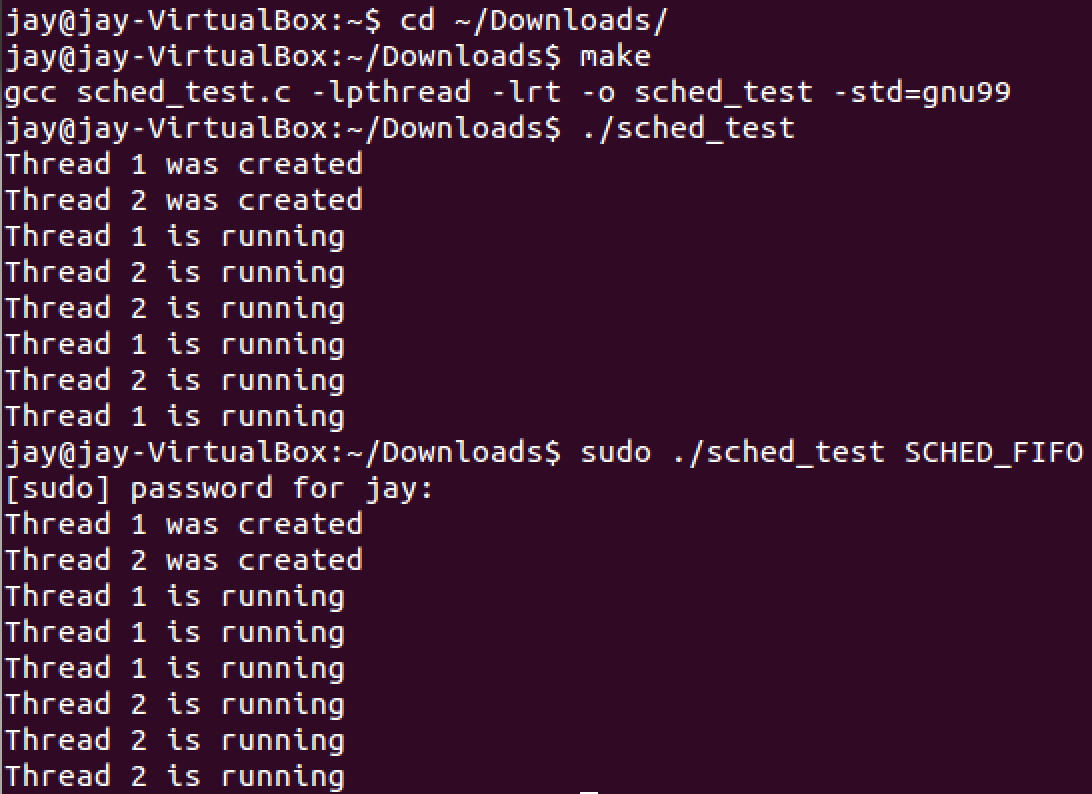
\includegraphics[width=0.5\textwidth]{img/sched_fifo.png}
\end{center}

\newpage
\subsection*{Part II: Weighted Round Robin Scheduler}

照著助教的提示後,解決了很多我們實作上的問題,花比較多時間主要是在查 function 功能、參數,以及 build kernel 的順序出了點問題,有很多細節應注意而未注意。\\

在執行時發現程式會卡在:

\begin{lstlisting}
if (sched_setscheduler(getpid(), sched_policy, &param) == -1)
\end{lstlisting}

但後來發現是自己電腦沒有打開多核心的設定,所以才沒有辦法順利地設定排程。

最後測試幾次輸出的結果:

\begin{center}
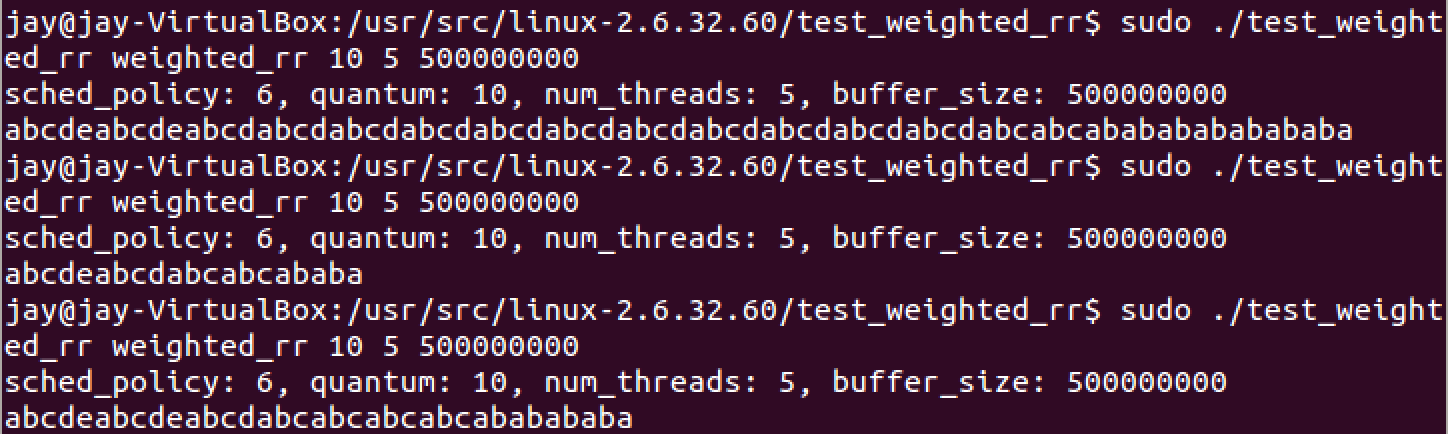
\includegraphics[width=1\textwidth]{img/sched_weighted_rr.png}
\end{center}

\end{document}